\documentclass{report}%
\usepackage[T1]{fontenc}%
\usepackage[utf8]{inputenc}%
\usepackage{textcomp}%
\usepackage{lastpage}%
\usepackage{geometry}%
\geometry{margin=0.5in,top=0.5in,bottom=0.5in}%
\usepackage{graphicx}%
%
\title{JMAG Complex Rotator Pipeline Results}%
\date{Generated on 06/16/25 11:29:26}%
\usepackage{float}%
\usepackage{hyperref}%
\hypersetup{colorlinks=true}%
%
\begin{document}%
\normalsize%
\maketitle%
\tableofcontents%
\chapter{Complex Rotators}%
\label{chap:ComplexRotators}%

%
\chapter{Non{-}Complex Rotators}%
\label{chap:Non{-}ComplexRotators}%
\newpage%
\section{TIC 68131578}%
\label{sec:TIC68131578}%
\subsection{Sector 91}%
\label{subsec:TIC6813157891}%


\begin{figure}[H]%
\begin{center}%
\centering%
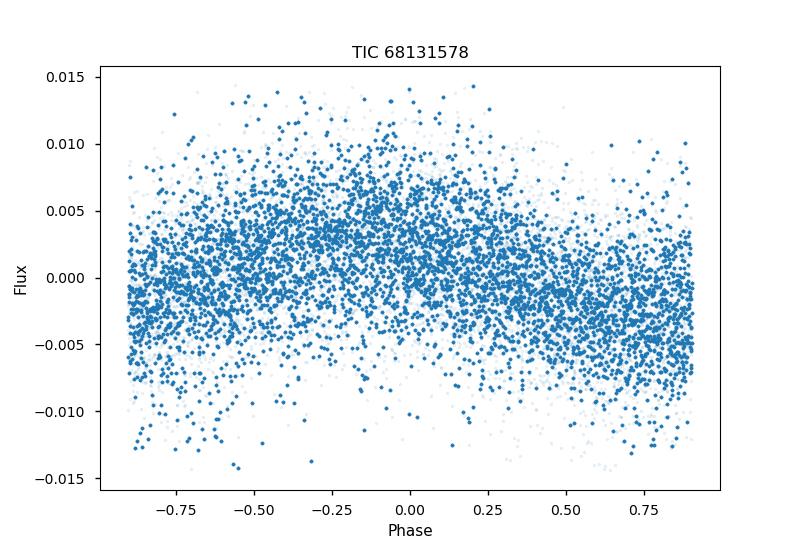
\includegraphics[width=0.5\textwidth]{/Users/sarahdraves/Library/CloudStorage/OneDrive-Personal/Documents/Research/BDNYC/SRMP-JMAG-Sarah/output/TIC 68131578/91_plot.png}%
\end{center}%
\end{figure}

%


\begin{figure}[H]%
\begin{center}%
\centering%
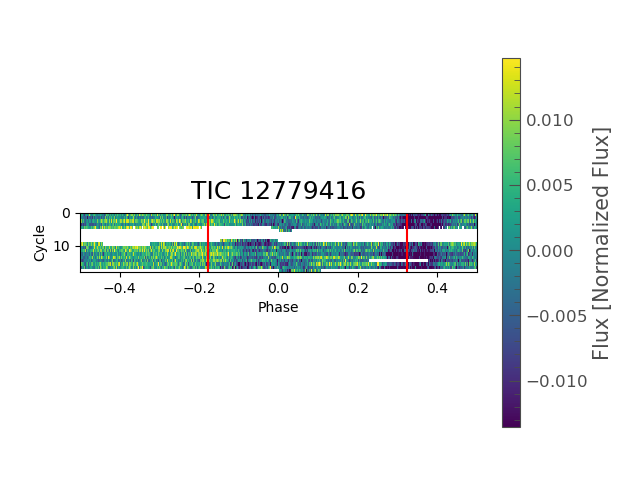
\includegraphics[width=0.5\textwidth]{/Users/sarahdraves/Library/CloudStorage/OneDrive-Personal/Documents/Research/BDNYC/SRMP-JMAG-Sarah/output/TIC 68131578/91_river.png}%
\end{center}%
\end{figure}

%


\begin{figure}[H]%
\begin{center}%
\centering%
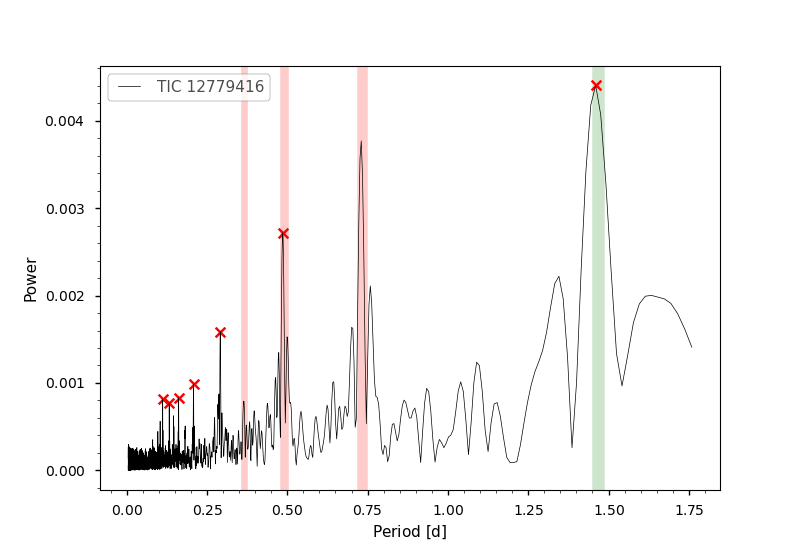
\includegraphics[width=0.5\textwidth]{/Users/sarahdraves/Library/CloudStorage/OneDrive-Personal/Documents/Research/BDNYC/SRMP-JMAG-Sarah/output/TIC 68131578/91_periodogram.png}%
\end{center}%
\end{figure}

%
\end{document}